\documentclass[../../main.tex]{subfiles}
\begin{document}

{\bf [解]}

\paragraph{(1)}

$f$ によって 点$(x, y)$ が 点$(X, Y)$ にうつるとすると
\begin{align}
  \begin{cases}
    X = 3x + y \\
    Y = -2x
  \end{cases}
  \quad \therefore
  \begin{cases}
    x = -\dfrac{1}{2}Y \\
    y = X + \dfrac{3}{2}Y
  \end{cases} \label{eq:1}
\end{align}
である．
従って$a_n x + b_n y = 1$ は，$a_n \left(-\dfrac{1}{2}Y\right) + b_n \left(X + \dfrac{3}{2}Y\right) = 1$ にうつるので係数を比較して，
\begin{align}
  \begin{cases}
    a_{n+1} = b_n \\
    b_{n+1} = -\dfrac{1}{2}a_n + \dfrac{3}{2}b_n
  \end{cases} \label{eq:2}
\end{align}
である．これが求める漸化式である．

\paragraph{(2)}

初期条件は題意より
\begin{align}
  a_0 = 3, b_0 = 2 \label{eq:3}
\end{align}
である．
\cref{eq:2}から$b_n$を消去すると
\begin{align}
  a_{n+2} = \dfrac{3}{2}a_{n+1} - \dfrac{1}{2}a_n
\end{align}
なので，これを\cref{eq:3}より$a_0=3, a_1=2$と合わせて解くと
\begin{align}
  a_n = 1 + \left(\dfrac{1}{2}\right)^{n-1} \label{eq:4}
\end{align}
である．従って(1)から直線$l_n$の方程式は
\begin{align}
  l_n : \left\{1+\left(\dfrac{1}{2}\right)^{n-1}\right\}x + \left\{1+\left(\dfrac{1}{2}\right)^n\right\}y = 1 \label{eq:5}
\end{align}
である．これを$l_0$と合わせて図示すると下図である．

% TODO: l_0と一般のl_nの図示
\begin{figure}[htb]
  \centering
  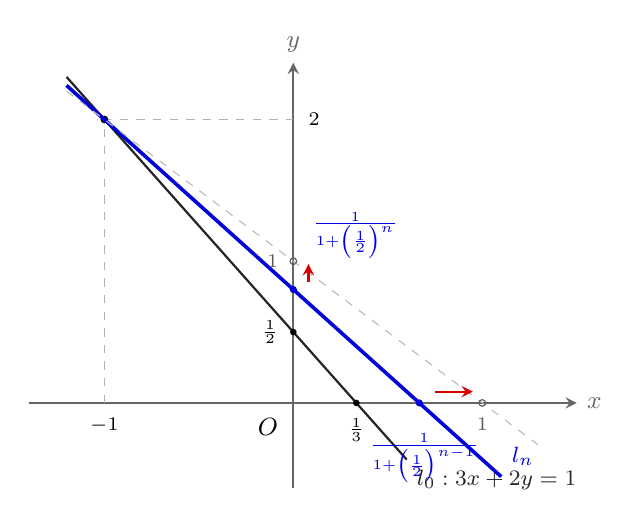
\begin{tikzpicture}[x=2.4cm, y=1.8cm, >=stealth, every node/.style={font=\small}]

    % --- 1. 座標定義 ---
    \coordinate (O) at (0, 0);
    \coordinate (Q) at (-1, 2); % 共通交点 (-1, 2)

    % --- 2. 座標軸 ---
    \draw[->, thick, gray!80!black] (-1.4, 0) -- (1.5, 0) node[right] {$x$};
    \draw[->, thick, gray!80!black] (0, -0.6) -- (0, 2.4) node[above] {$y$};
    \node[below left=2pt] at (O) {$O$};

    % --- 3. 共通交点 Q(-1, 2) の補助点線 ---
    \draw[dashed, gray!60] (-1, 0) -- (Q) -- (0, 2);
    \node[below=2pt, font=\scriptsize] at (-1, 0) {$-1$};
    \node[right=2pt, font=\scriptsize] at (0, 2) {$2$};
    \fill[black] (Q) circle (1.4pt);

    % --- 4. 直線 l_0: 3x + 2y = 1 ---
    % 切片: x = 1/3, y = 1/2
    \draw[thick, gray!30!black] (-1.2, 2.3) -- (0.6, -0.4)
    node[below right, font=\footnotesize] {$l_0: 3x+2y=1$};

    % --- 5. 直線 l_n (n = 2 の厳密プロット: y = -1.2*x + 0.8) ---
    \draw[line width=1.3pt, blue!85!black] (-1.2, 2.24) -- (1.1, -0.52)
    node[above right, font=\footnotesize\bfseries] {$l_n$};

    % --- 6. 極限直線 l_infty: x + y = 1 (点線) ---
    \draw[dashed, gray!55] (-1.2, 2.2) -- (1.3, -0.3);

    % --- 7. 切片のプロットと移動矢印 ---
    % l_0 の切片
    \fill[black] (1/3, 0) circle (1.2pt) node[below=2pt, font=\scriptsize] {$\frac{1}{3}$};
    \fill[black] (0, 0.5) circle (1.2pt) node[left=2pt, font=\scriptsize] {$\frac{1}{2}$};

    % l_n の切片
    \fill[blue!85!black] (2/3, 0) circle (1.3pt);
    \fill[blue!85!black] (0, 0.8) circle (1.3pt);

    % 切片のラベル（引き出し線）
    \node[font=\scriptsize, blue!90!black, below right] at (0.35, -0.15)
    {$\frac{1}{1 + \left(\frac{1}{2}\right)^{n-1}}$};
    \node[font=\scriptsize, blue!90!black, above right] at (0.05, 0.95)
    {$\frac{1}{1 + \left(\frac{1}{2}\right)^n}$};

    % 極限値 1 の白丸と矢印
    \draw[gray!70!black] (1, 0) circle (1.2pt) node[below=2pt, font=\scriptsize] {$1$};
    \draw[gray!70!black] (0, 1) circle (1.2pt) node[left=2pt, font=\scriptsize] {$1$};

    % 移動方向の矢印
    \draw[->, thick, red!85!black] (0.75, 0.08) -- (0.95, 0.08);
    \draw[->, thick, red!85!black] (0.08, 0.85) -- (0.08, 0.98);

  \end{tikzpicture}
  \caption{直線 $l_0$ と一般の直線 $l_n$}
  \label{fig:line_ln_movement}
\end{figure}

さて，$x,y$切片である$1+\left(\dfrac{1}{2}\right)^{n-1}, 1+\left(\dfrac{1}{2}\right)^n$ は $n$ について単調に増加し，$n\to\infty$で共に 1 に収束する．
$l_n$ と $l_{0}$ の交点 $Q_n$ は$n$にかかわらず $Q_n(-1, 2)$ であり，$l_n$ の傾きを
\begin{align}
  C_n = -\dfrac{1+\left(\dfrac{1}{2}\right)^{n-1}}{1+\left(\dfrac{1}{2}\right)^n}
\end{align}
とすると，簡単のため$\alpha = \dfrac{1}{2}$ として
\begin{align}
  \dfrac{-C_n}{-C_{n+1}} = \dfrac{\alpha^{2n} + \dfrac{5}{4}\alpha^n + 1}{\alpha^{2n} + 2\alpha^n + 1} < 1 \quad \therefore C_n < C_{n+1}
\end{align}
だから，$C_n$ は単調増加で，$C_1 = -\dfrac{3}{2}, C_n \to -1 \, (n \to \infty)$ となる．以上から$l_n$ は$l_0$と
\begin{align}
  \lim_{n\to\infty}l_n: x+y=1
\end{align}
の間を動く．これを図示すると下図の斜線部（境界は実線のみ含む）である．

% TODO: l_0とl_inftyの間の領域の図示
\begin{figure}[htb]
  \centering
  \begin{tikzpicture}[x=2.2cm, y=1.6cm, >=stealth, every node/.style={font=\small}]

    % --- 1. 座標定義 ---
    \coordinate (O) at (0, 0);
    \coordinate (Q) at (-1, 2);

    % --- 2. 直線 l_0 と l_infty の通過領域（斜線部） ---
    % (i) 第 1 象限側 (x > -1)
    \fill[pattern=north east lines, pattern color=blue!75, opacity=0.8]
    (Q) -- (1.5, -1.75) -- (1.5, -0.5) -- cycle;

    % (ii) 第 2 象限奥側 (x < -1)
    \fill[pattern=north east lines, pattern color=blue!75, opacity=0.8]
    (Q) -- (-1.5, 2.75) -- (-1.5, 2.5) -- cycle;

    % --- 3. 座標軸 ---
    \draw[->, thick, gray!80!black] (-1.8, 0) -- (1.8, 0) node[right] {$x$};
    \draw[->, thick, gray!80!black] (0, -1.2) -- (0, 3.0) node[above] {$y$};
    \node[below left=2pt] at (O) {$O$};

    % --- 4. 2本の境界直線 ---
    % l_0: 3x + 2y = 1  => y = -1.5x + 0.5 (実線)
    \draw[line width=1.3pt, gray!20!black] (-1.5, 2.75) -- (1.5, -1.75)
    node[below right, font=\footnotesize] {$3x+2y=1$};

    % l_infty: x + y = 1 => y = -x + 1 (破線)
    \draw[line width=1.3pt, gray!40!black, dashed] (-1.5, 2.5) -- (1.5, -0.5)
    node[above right, font=\footnotesize] {$x+y=1$};

    % --- 5. 補助線・目盛り ---
    \draw[dashed, gray!60] (-1, 0) -- (Q) -- (0, 2);
    \node[below=2pt, font=\scriptsize] at (-1, 0) {$-1$};
    \node[right=2pt, font=\scriptsize] at (0, 2) {$2$};

    \fill[black] (Q) circle (1.5pt);
    \node[left=1pt, font=\scriptsize] at (Q) {$(-1,2)$};

    \fill[black] (1/3, 0) circle (1.2pt) node[below=2pt, font=\scriptsize] {$\frac{1}{3}$};
    \fill[black] (1, 0)   circle (1.2pt) node[below=2pt, font=\scriptsize] {$1$};

  \end{tikzpicture}
  \caption{直線 $l_n$ が動く通過領域（$l_0$ と $l_\infty$ の間）}
  \label{fig:ln_sweep_region}
\end{figure}

従って，全ての$n$について$a_n x+b_ny > 1$となる領域は下図の斜線部（境界は実線のみ含む）である．

% TODO: 求めうる領域の図示
\begin{figure}[htb]
  \centering
  \begin{tikzpicture}[x=2.2cm, y=1.6cm, >=stealth, every node/.style={font=\small}]

    % --- 1. 座標定義 ---
    \coordinate (O) at (0, 0);
    \coordinate (Q) at (-1, 2);

    % ============================================================
    % 2. 求める共通領域の斜線塗りつぶし (手書きスケッチ3)
    % 領域: 3x+2y > 1 (x < -1) かつ x+y >= 1 (x >= -1)
    % ============================================================
    \fill[pattern=north east lines, pattern color=blue!75, opacity=0.8]
    (-1.5, 3.2) -- (-1.5, 2.75) -- (Q) -- (1.5, -0.5) -- (1.5, 3.2) -- cycle;

    % ============================================================
    % 3. 座標軸
    % ============================================================
    \draw[->, thick, gray!80!black] (-1.8, 0) -- (1.8, 0) node[right] {$x$};
    \draw[->, thick, gray!80!black] (0, -0.8) -- (0, 3.2) node[above] {$y$};
    \node[below left=2pt] at (O) {$O$};

    % ============================================================
    % 4. 境界直線
    % ============================================================
    % (1) 境界の実線部（領域の境界をなす半直線）
    \draw[line width=1.5pt, gray!20!black] (-1.5, 2.75) -- (Q); % 3x+2y=1 (x <= -1)
    \draw[line width=1.5pt, gray!20!black] (Q) -- (1.5, -0.5);  % x+y=1    (x >= -1)

    % (2) 領域の境界でない部分（破線）
    \draw[dashed, gray!50, line width=1.0pt] (Q) -- (1.2, -1.3); % 3x+2y=1 の続き
    \draw[dashed, gray!50, line width=1.0pt] (-1.5, 2.5) -- (Q); % x+y=1 の続き

    % ラベル
    \node[below right, font=\footnotesize] at (1.2, -1.3) {$3x+2y=1$};
    \node[above right, font=\footnotesize] at (1.5, -0.5)  {$x+y=1$};

    % ============================================================
    % 5. 補助線と目盛り
    % ============================================================
    \draw[dashed, gray!60] (-1, 0) -- (Q) -- (0, 2);
    \node[below=2pt, font=\scriptsize] at (-1, 0) {$-1$};
    \node[right=2pt, font=\scriptsize] at (0, 2) {$2$};

    % 切片目盛り
    \fill[black] (1/3, 0) circle (1.2pt) node[below=2pt, font=\scriptsize] {$\frac{1}{3}$};
    \fill[black] (1, 0)   circle (1.2pt) node[below=2pt, font=\scriptsize] {$1$};
    \fill[black] (0, 0.5) circle (1.2pt) node[left=2pt, font=\scriptsize] {$\frac{1}{2}$};

    % 点 (-1, 2) の白丸（共通交点）
    \fill[white] (Q) circle (2.2pt);
    \draw[thick, black] (Q) circle (2.2pt);

  \end{tikzpicture}
  \caption{すべての $n$ について $a_n x + b_n y > 1$ を満たす領域（斜線部）}
  \label{fig:intersection_halfplanes_region}
\end{figure}

\end{document}
